\section{Introduction}
\label{sec:intro}

Federated fine-tuning enables multiple clients to adapt a pretrained language
model collaboratively while keeping their private data decentralized.
Combined with parameter-efficient adaptation such as LoRA~\cite{hu2022lora},
federated fine-tuning avoids transmitting the full language model and has been
used to adapt large language models to decentralized instruction and task data
without collecting raw client examples~\cite{mcmahan2017fedavg,zhang2024fedit,sun2024ffalora}.

The standard approach gives every client a LoRA adapter with the same rank and
aggregates the corresponding factors across clients \cite{zhang2024fedit}.
However, clients in a federated deployment may have substantially different
memory, compute, and communication budgets \TODO{refs}.
Assigning the same LoRA rank to all clients either exceeds the resources of
constrained clients or leaves the capacity of stronger clients underused.
A natural way to accommodate this resource heterogeneity is to assign client
$i$ a fixed rank budget $r_i$ and let clients fine-tune adapters with different
ranks~\cite{bai2024flexlora,wang2024flora,cho2024hetlora}.
This change makes cross-client aggregation nontrivial: although the effective
updates $B_iA_i$ have the same output shape, the factor matrices have
rank-dependent inner dimensions and cannot be directly averaged.

Existing rank-heterogeneous methods resolve this incompatibility by introducing
additional server-side operations, but they incur important trade-offs, 
\eg high communication cost~\cite{wang2024flora} or lack of fairness guarantees across clients~\cite{bai2024flexlora}.
In this paper, we explore \textit{Selective Rank Sharing}, a simple and
communication-efficient approach to rank-heterogeneous federated LoRA
fine-tuning.
As shown in \figref{fig:selective-rank-sharing}, each client partitions its fixed rank budget into a globally shared prefix and a client-specific protected remainder.
Only the shared prefix is aggregated and broadcast, while both portions remain trainable locally.
This design preserves each client's total rank budget and avoids requiring
full-size adapter communication or server-side SVD for rank redistribution.

We further conduct motivation experiments on FLAN~\cite{wei2022finetuned} with eight clients, assigning fixed rank budgets of 16 and 64 to four clients each (see \figref{fig:acl-motivation}).
The experiments reveal two observations.
\textit{(i)} Changing the shared-prefix width affects rank groups differently: a
width that improves one group can hurt another, and the same width consumes
different fractions of clients' rank budgets.
\textit{(ii)} At a fixed shared width, the relative cosine similarity of same-rank and same-domain updates varies across the two rank groups and training rounds.
These geometric differences leave open how external updates affect each client's task performance.
These observations lead to the following two challenges.

\begin{figure}[!t]
    \centering
    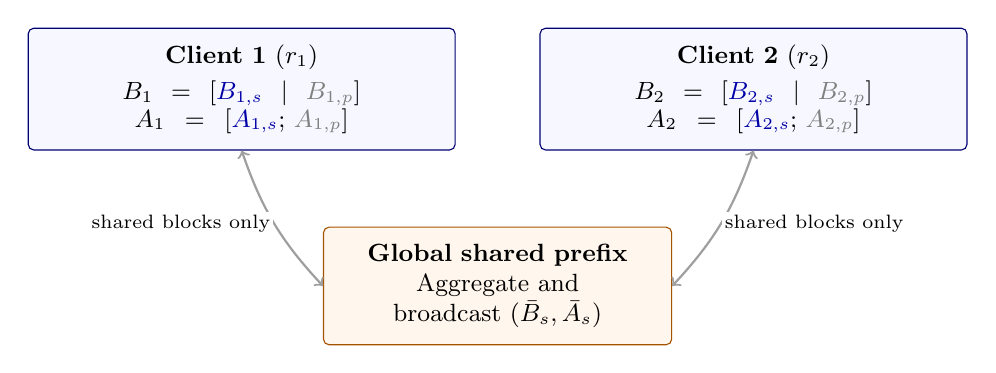
\begin{tikzpicture}[
        client/.style={draw=blue!45!black, fill=blue!3, rounded corners=2pt,
            text width=5.0cm, align=center, inner sep=6pt, font=\small},
        server/.style={draw=orange!65!black, fill=orange!7, rounded corners=2pt,
            text width=4.0cm, align=center, inner sep=6pt, font=\small},
        sync/.style={<->, thick, draw=gray!75}
    ]
        \node[client] (client1) at (-3.25,1.35) {\textbf{Client 1} ($r_1$)\\[2pt]
            $B_1=[\textcolor{blue!65!black}{B_{1,s}}\mid\textcolor{gray}{B_{1,p}}]$\\[-1pt]
            $A_1=[\textcolor{blue!65!black}{A_{1,s}};\,\textcolor{gray}{A_{1,p}}]$};
        \node[client] (client2) at (3.25,1.35) {\textbf{Client 2} ($r_2$)\\[2pt]
            $B_2=[\textcolor{blue!65!black}{B_{2,s}}\mid\textcolor{gray}{B_{2,p}}]$\\[-1pt]
            $A_2=[\textcolor{blue!65!black}{A_{2,s}};\,\textcolor{gray}{A_{2,p}}]$};
        \node[server] (global) at (0,-1.15) {\textbf{Global shared prefix}\\
            Aggregate and broadcast $(\bar{B}_{s},\bar{A}_{s})$};
        \draw[sync] (client1.south) to[bend right=12]
            node[midway,left,font=\scriptsize,fill=white,inner sep=1pt] {shared blocks only}
            (global.west);
        \draw[sync] (client2.south) to[bend left=12]
            node[midway,right,font=\scriptsize,fill=white,inner sep=1pt] {shared blocks only}
            (global.east);
    \end{tikzpicture}
    \caption{Selective Rank Sharing. For heterogeneous clients with $r_1\ne r_2$, blue denotes the shared prefix of width $s$, while gray denotes each client's remainder of width $p_i=r_i-s$. \TODO{replace it}}
    \label{fig:selective-rank-sharing}
\end{figure}
\FloatBarrier

\begin{itemize}
    \item \textbf{How should a global receiving width be selected under heterogeneous rank budgets?}
    A fixed shared width gives all clients the same receiving capacity even
    though it occupies different proportions of their fixed rank budgets and
    can have opposite effects on different rank groups.

    \item \textbf{How should the influence of external updates be adapted under coupled data and structural heterogeneity?}
    Clients differ in both their local data and their adapter rank, so the
    relationship between updates is client- and round-dependent.
    A collaboration mechanism must therefore determine which external
    influence is useful to a client and how strongly it should be applied.
\end{itemize}

The two challenges are coupled: the selected receiving width determines the
subspace in which external knowledge can enter, while the usefulness of that
knowledge affects whether the selected width is worthwhile.
To solve the coupled challenges, we propose \sysname, a federated LoRA fine-tuning framework that
\TODO{Introduce the complete method and map its components to the two challenges.}

\TODO{Summarize the contributions.}


\begin{figure}[t]
    \centering
    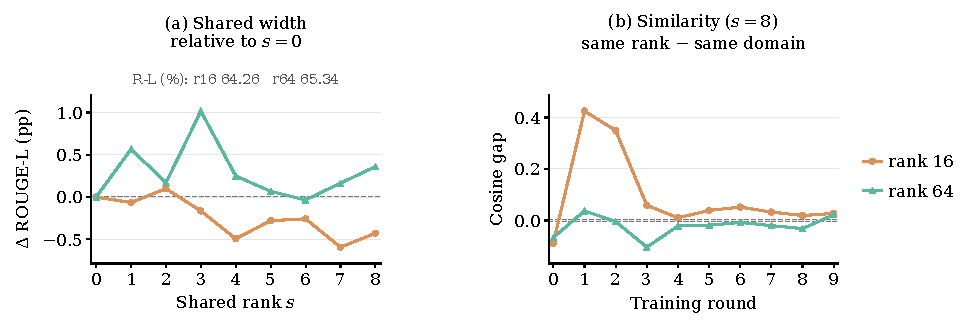
\includegraphics[width=0.8\linewidth]{figs/acl_motivation_flan_r16_64.pdf}
    \caption{Selective rank sharing on FLAN with eight clients and two rank budgets, 16 and 64 (four clients each), under Dirichlet $\alpha=0.5$.
    (a) Rank-group ROUGE-L changes as the shared-prefix width $s$ varies, relative to each group's matched $s=0$ run; the corresponding absolute ROUGE-L scores are shown above the panel.
    At $s=8$, ROUGE-L decreases for rank 16 and increases for rank 64.
    (b) In an independent $s=8$ run, we plot the mean cosine of effective shared-upload changes for same-rank/different-domain pairs minus that for same-domain/different-rank pairs over R0--R9.
    The two rank groups exhibit different alignment trajectories; diagnostic details are given in \appref{sec:appendix:motivation-setup}.}
    \label{fig:acl-motivation}
\end{figure}
